\documentclass[a4paper,%
7pt,%
DIV12,
headsepline,%
headings=normal,
]{scrartcl}

\usepackage[parfill]{parskip}

\usepackage{./docs/bopc}
\usepackage{csvsimple}
\usepackage{listings}
\usepackage{booktabs}
\usepackage{array}
\usepackage[utf8]{inputenc}
\usepackage{pmboxdraw}


%% ==================== ADAPT ACCORDINGLY ==================== %%

% args: first name, last name, matriculation number
\setAuthorOne{Pia}{Schwarzinger}{12017370}
\setAuthorTwo{Yahya}{Jabary}{11912007}

% set group size and group number, group size influences author formatting

% args: group size, group number (TUWEL)
\setGroup{2}{13}

%% =========================================================== %%

\begin{document}

\maketitlepage

%% ================= SUBMISSION INFORMATION ================== %%

% Please fill out accordingly

%% ========================= REPORT ========================== %%

\section{Exercise 1}

\lstinputlisting{./demo/scheduler.c}

\subsection{What do \texttt{a} and \texttt{t} count?}

The variable \texttt{a} stores the selected thread number for each parallel iteration, while \texttt{t} stores a non-atomic counter that all threads with the same ID increment. Unless no two threads are assigned the same iteration, the final value of \texttt{t} will be non-deterministic as each \texttt{var++} operation is in fact a read-modify-write operation:

\begin{verbatim}
movl  -4(%rbp), %eax   # load var into eax
addl  $1, %eax         # increment eax by 1
movl  %eax, -4(%rbp)   # store eax back into var
\end{verbatim}

\subsection{Values for all elements in \texttt{a} and \texttt{t}}

See Tables \ref{tab:values_a} and \ref{tab:values_t} for the values of \texttt{a} and \texttt{t} for different scheduling strategies.

\begin{table}[htbp]
    \centering
    \caption{Values of array \texttt{a} for different scheduling strategies}
    \label{tab:values_a}
    \begin{tabular}{l*{17}{c}}
        \toprule
        case / \texttt{a} & 0 & 1 & 2 & 3 & 4 & 5 & 6 & 7 & 8 & 9 & 10 & 11 & 12 & 13 & 14 & 15 & 16 \\
        \midrule
        \texttt{static, 0} & 0 & 0 & 0 & 0 & 0 & 0 & 1 & 1 & 1 & 1 & 1 & 1 & 2 & 2 & 2 & 2 & 2 \\
        \texttt{static, 1} & 0 & 1 & 2 & 0 & 1 & 2 & 0 & 1 & 2 & 0 & 1 & 2 & 0 & 1 & 2 & 0 & 1 \\
        \texttt{dynamic, 1} & 1 & 1 & 1 & 1 & 1 & 1 & 1 & 1 & 1 & 1 & 1 & 1 & 1 & 1 & 1 & 1 & 1 \\
        \texttt{dynamic, 2} & 0 & 0 & 0 & 0 & 0 & 0 & 0 & 0 & 0 & 0 & 0 & 0 & 0 & 0 & 0 & 0 & 0 \\
        \texttt{guided, 5} & 0 & 0 & 0 & 0 & 0 & 0 & 0 & 0 & 0 & 0 & 0 & 0 & 0 & 0 & 0 & 0 & 0 \\
        \bottomrule
    \end{tabular}
\end{table}

\begin{table}[htbp]
    \centering
    \caption{Values of array \texttt{t} for different scheduling strategies - keep in mind that these values are not reproducible / deterministic.}
    \label{tab:values_t}
    \begin{tabular}{l*{3}{c}}
        \toprule
        case / \texttt{t} & 0 & 1 & 2 \\
        \midrule
        \texttt{static, 0} & 74307862 & 7 & 1806905557 \\
        \texttt{static, 1} & 8591638 & 7 & 1872621781 \\
        \texttt{dynamic, 1} & 6150416 & 18 & 1875062992 \\
        \texttt{dynamic, 2} & 40737057 & 1 & 1840476368 \\
        \texttt{guided, 5} & 51370273 & 1 & 1829843168 \\
        \bottomrule
    \end{tabular}
\end{table}

\section{Exercise 2}

\begin{table}[htbp]
    \centering
    \caption{Duration of independent tasks we want to schedule optimally.}
    \label{tab:task_duration}
    \begin{tabular}{l*{17}{c}}
        \toprule
        Task ID & 0 & 1 & 2 & 3 & 4 & 5 & 6 & 7 & 8 & 9 & 10 & 11 & 12 & 13 & 14 & 15 & 16 \\
        \midrule
        Task duration & 1 & 2 & 1 & 2 & 1 & 2 & 1 & 2 & 1 & 2 & 1 & 2 & 1 & 2 & 4 & 3 & 3 \\
        \bottomrule
    \end{tabular}
\end{table}

\subsection{Optimal Schedule}

To minimize the total execution time with 4 workers, we can use the ``Longest Processing Time'' (LPT) algorithm by R. L. Graham in 1969. Here's how it works: First, sort the tasks by duration in descending order. Then, assign the tasks to the least loaded worker. But beware that the LPT isn't guaranteed to find the optimal solution, but just to have a provable upper bound of $\lceil 4/3 \cdot \text{OPT} \rceil$ where OPT is the optimal solution.

Assuming that tasks can be interrupted and resumed at any time, we can calculate the OTP as follows: $\text{OPT} = \lceil \sum_{i=0}^{16} \text{task duration}_i / 4 \rceil = \lceil 31 / 4 \rceil = 8$.

Fortunately we were able to find one of the optimal solutions by using the LPT algorithm.

\lstinputlisting{./demo/scheduler.py}

\begin{verbatim}
sorted tasks: [4, 3, 3, 2, 2, 2, 2, 2, 2, 2, 1, 1, 1, 1, 1, 1, 1]

worker 0:
        task 14, start: 0, end: 4 (duration: 4)
        task 9, start: 4, end: 6 (duration: 2)
        task 2, start: 6, end: 7 (duration: 1)
        task 8, start: 7, end: 8 (duration: 1)

worker 1:
        task 15, start: 0, end: 3 (duration: 3)
        task 5, start: 3, end: 5 (duration: 2)
        task 13, start: 5, end: 7 (duration: 2)
        task 10, start: 7, end: 8 (duration: 1)

worker 2:
        task 16, start: 0, end: 3 (duration: 3)
        task 7, start: 3, end: 5 (duration: 2)
        task 0, start: 5, end: 6 (duration: 1)
        task 4, start: 6, end: 7 (duration: 1)
        task 12, start: 7, end: 8 (duration: 1)

worker 3:
        task 1, start: 0, end: 2 (duration: 2)
        task 3, start: 2, end: 4 (duration: 2)
        task 11, start: 4, end: 6 (duration: 2)
        task 6, start: 6, end: 7 (duration: 1)

time spent: 8
\end{verbatim}

\begin{figure}[htbp]
    \centering
    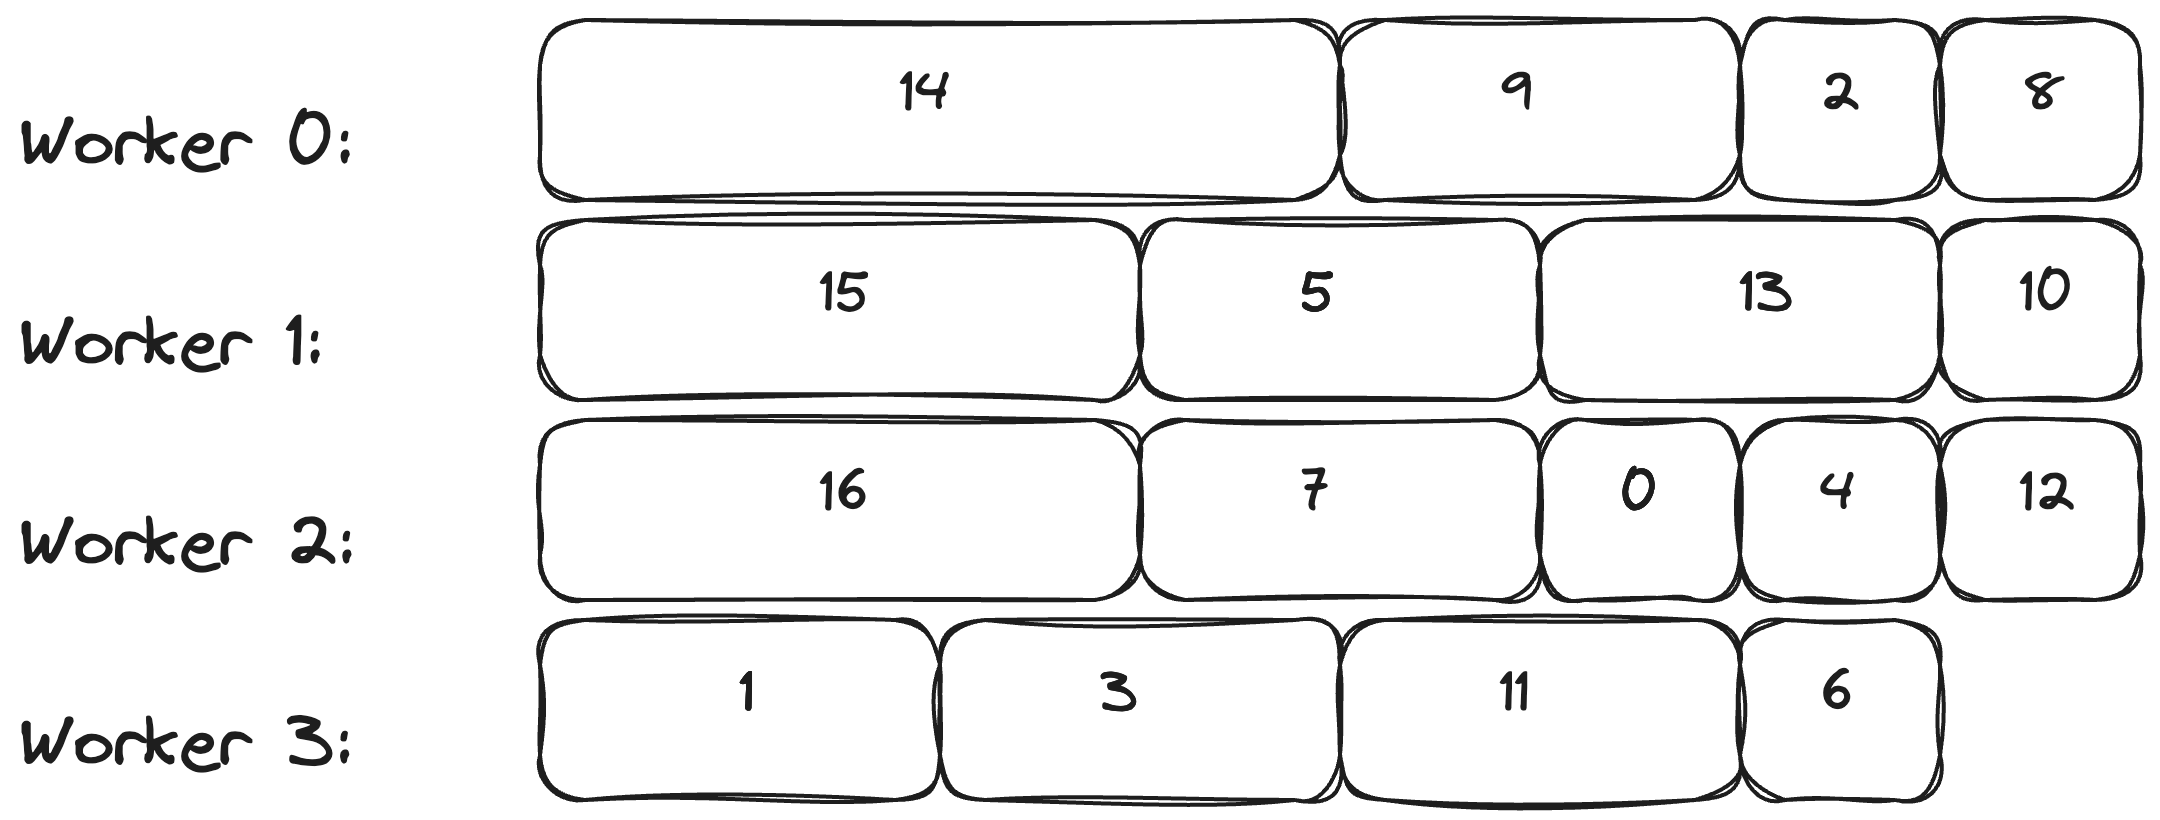
\includegraphics[width=0.75\textwidth]{./assets/gantt_lpt.png}
    \caption{Gantt chart of the LPT schedule (which happens to be optimal).}
    \label{fig:gantt_lpt}
\end{figure}

\subsection{Schedule \texttt{static,3}}

The schedule \texttt{static,3} assigns each task to a worker in a round-robin fashion with a chunk size of 3.

The makespan of the schedule \texttt{static,3} is 11, which is suboptimal compared to the LPT schedule. The Gantt chart in Figure \ref{fig:gantt_static3} shows the schedule.

\begin{figure}[htbp]
    \centering
    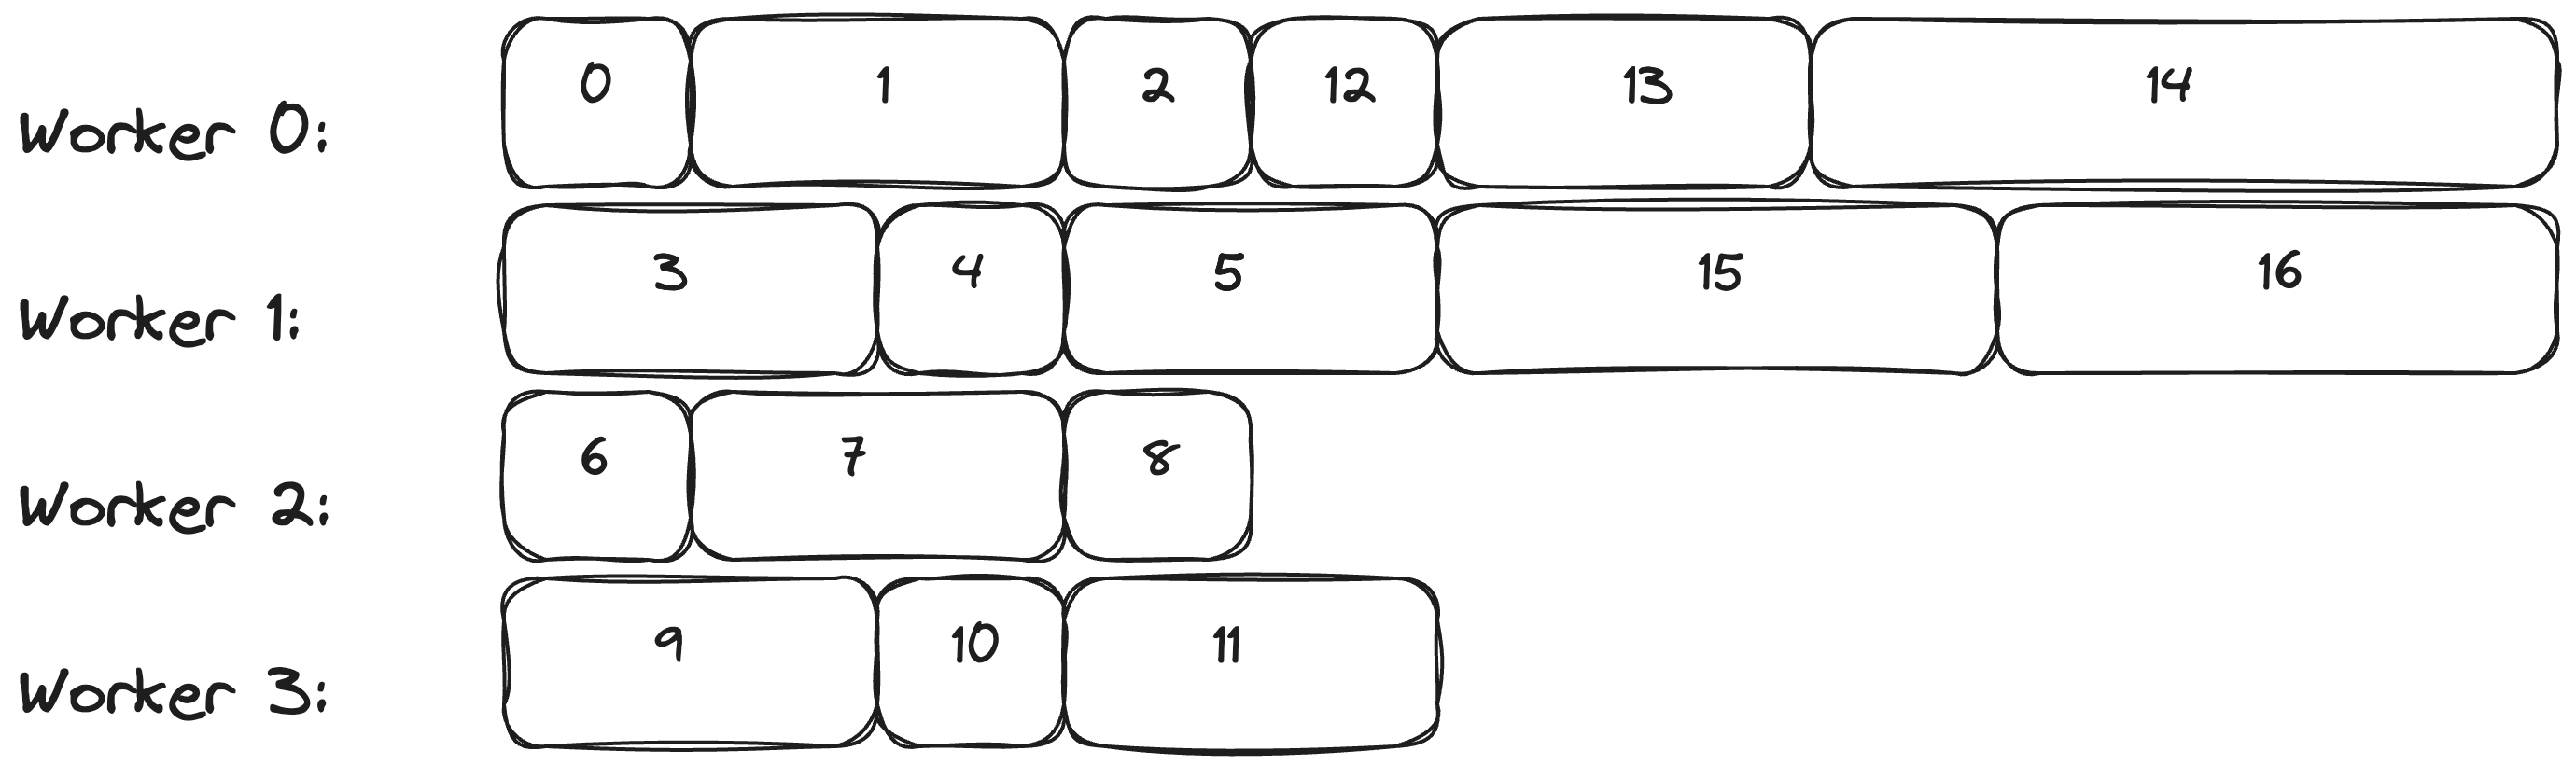
\includegraphics[width=0.75\textwidth]{./assets/static3.png}
    \caption{Gantt chart of the schedule \texttt{static,3}.}
    \label{fig:gantt_static3}
\end{figure}

\subsection{Schedule \texttt{dynamic,2}}

The schedule \texttt{dynamic,2} assigns chunks of 2 tasks to a random worker that is currently idle.

The makespan of the schedule \texttt{dynamic,2} is 10, which is suboptimal compared to the LPT schedule but better than the \texttt{static,3} schedule. The Gantt chart in Figure \ref{fig:gantt_static3} shows the schedule.

\begin{figure}[htbp]
    \centering
    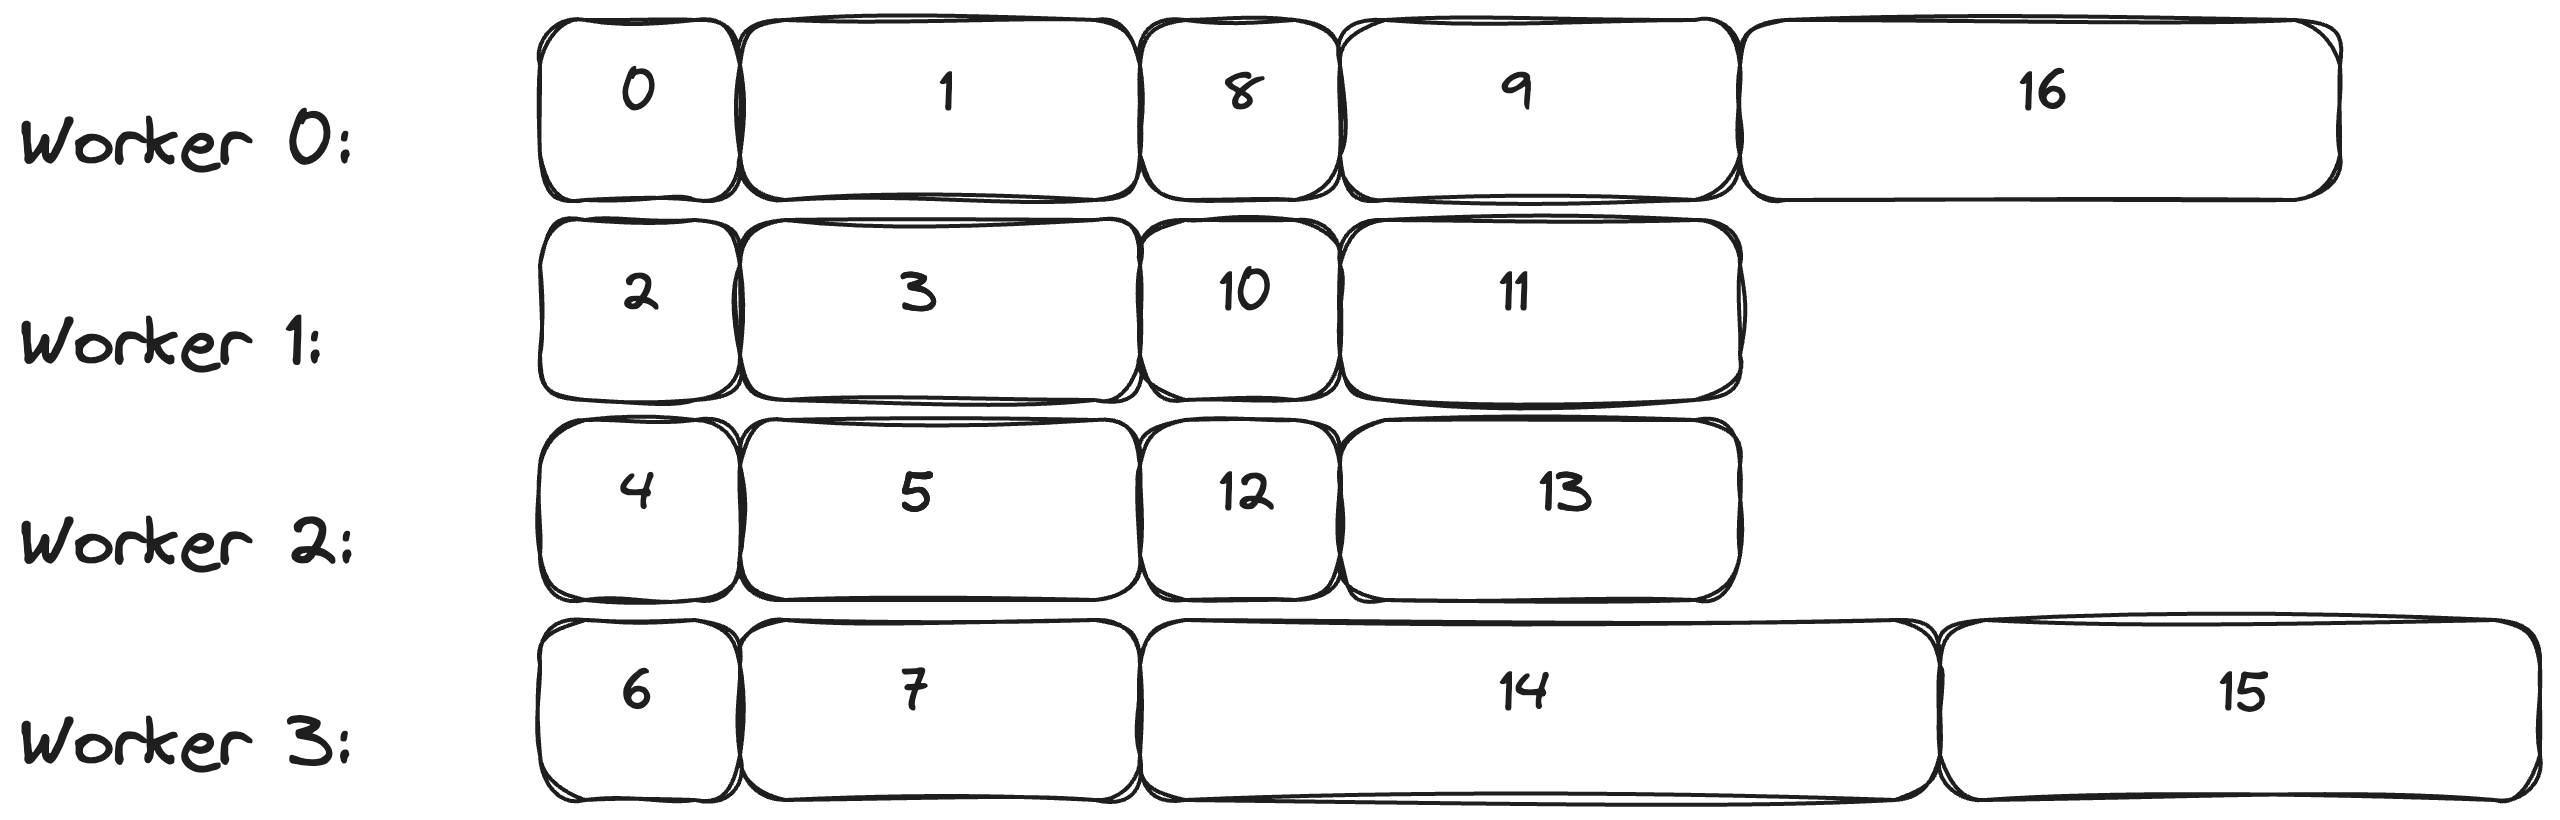
\includegraphics[width=0.75\textwidth]{./assets/dynamic2.png}
    \caption{Gantt chart of the schedule \texttt{dynamic,2}.}
    \label{fig:gantt_static3}
\end{figure}

\section{Exercise 3}

\subsection{Fix the problems with this OpenMP code}

Here are some suggestions to fix the problems with the given code snippet:

\begin{itemize}
    \item The instruction \texttt{count\_odd += my\_count\_odd;} doesn't make a lot of sense given that only the \texttt{\#pragma} region inside the \texttt{for} loop is parallelized. Replace the \texttt{my\_count\_odd} variable with the shared variable \texttt{count\_odd} and use an atomic operation to increment it. 

    \item Or even better: Use a reduction clause to sum up the number of odd numbers in the array instead of declaring a shared variable and incrementing it atomically yourself.
    
    \item Turn the function \texttt{static} so it's just visible in a single translation / compilation unit (optional).
\end{itemize}

\lstinputlisting{./demo/odd_counter.c}

\section{Exercise 4}

\subsection{What is the output of the three different versions?}

Here are the results of the 3 given versions of the code snippet when compiled with \texttt{gcc -fopenmp} and executed with \texttt{omp\_set\_num\_threads(4)}:

\begin{verbatim}
$ gcc -fopenmp -o version_a version_a.c && ./version_a
res=1

$ gcc -fopenmp -o version_b version_b.c && ./version_b
res=5

$ gcc -fopenmp -o version_c version_c.c && ./version_c
res=5
\end{verbatim}

The results differ because of the \texttt{shared} and \texttt{private} clauses in the \texttt{omp\_task} function. The \texttt{shared} clause is used to share the result of the sub-task with the parent task, while the \texttt{private} clause is used to create a local copy of the result for each thread.

Here's some ASCII art to illustrate the stack-trace in the case of one sub-task result being shared and the other being private:

\begin{verbatim}
v=5             -> final result: 1
├── v=4         -> shared: 1
|  ├── v=3      -> shared: 1
|  |  ├── v=2   -> shared: 1
|  |  └── v=1   -> private
|  └── v=2      -> private
└── v=3         -> private
    ├── v=2     -> shared: 1
    └── v=1     -> private
\end{verbatim}

And here's the stack-trace for the case where both sub-task results are shared:

\begin{verbatim}
v=5             -> final result: 5
├── v=4         -> shared: 3
|  ├── v=3      -> shared: 2
|  |  ├── v=2   -> shared: 1
|  |  └── v=1   -> shared: 1
|  └── v=2      -> shared: 1
└── v=3         -> shared: 2
    ├── v=2     -> shared: 1
    └── v=1     -> shared: 1
\end{verbatim}

\subsection{How often is the function \texttt{omp\_tasks} called?}

Let's add a print statement to the \texttt{omp\_tasks} function to see how often it is called / what values are passed to it.

This is the most straightforward way to print the stack-trace for our use case. I also tried to write a custom \texttt{lldb} python script and a bunch of C-libraries to achieve the same result, but they all failed when combined with the OpenMP runtime.

Here are the modified versions of the code snippets:

\lstinputlisting{./demo/compare1.c}

\lstinputlisting{./demo/compare2.c}

\lstinputlisting{./demo/compare3.c}

And here's the output of the modified scripts:

\begin{verbatim}
$ gcc -fopenmp -o version_a version_a.c && ./version_a
called with v=5
called with v=3
called with v=4
called with v=1
called with v=3
called with v=2
called with v=2
called with v=1
called with v=2
res=1

$ gcc -fopenmp -o version_a version_a.c && ./version_a | grep -c "called with v" | xargs echo "num calls:"
num calls: 9

$ gcc -fopenmp -o version_b version_b.c && ./version_b
called with v=5
called with v=3
called with v=1
called with v=4
called with v=2
called with v=3
called with v=1
called with v=2
called with v=2
res=5

$ gcc -fopenmp -o version_b version_b.c && ./version_b | grep -c "called with v" | xargs echo "num calls:"
num calls: 9

$ gcc -fopenmp -o version_c version_c.c && ./version_c
called with v=5
called with v=3
called with v=1
called with v=2
called with v=4
called with v=2
called with v=3
called with v=1
called with v=2
called with v=5
called with v=3
called with v=1
called with v=2
called with v=4
called with v=2
called with v=3
called with v=1
called with v=2
called with v=5
called with v=3
called with v=1
called with v=2
called with v=4
called with v=3
called with v=1
called with v=2
called with v=2
called with v=5
called with v=3
called with v=1
called with v=2
called with v=4
called with v=2
called with v=3
called with v=1
called with v=2
res=5

$ gcc -fopenmp -o version_c version_c.c && ./version_c | grep -c "called with v" | xargs echo "num calls:"
num calls: 36
\end{verbatim}

We've already discussed the effect the inner \texttt{shared} and \texttt{private} clauses have on the final result. The number of calls to the \texttt{omp\_tasks} function however depends on the the pragma used in the \texttt{main} function:

\begin{itemize}

    \item Version A / \texttt{master}: This pragma causes the recursive function to be called from the \texttt{main} function just once. The \texttt{master} pragma ensures that only the master thread executes the critical section.

    \item Version B / \texttt{single nowait}: The \texttt{single} pragma ensures that only one thread executes the critical section, while the \texttt{nowait} clause allows the thread to continue executing the next section of code without waiting for the other threads to finish. The \texttt{nowait} clause in this case doesn't have any effect as it is the last section of code in the \texttt{parallel} region of the \texttt{main} function.
    
    \item Version C / \texttt{critical}: This pragma caused the recursive function to be executed 36 (4 threads $\cdot$ 9 recursive calls) times. The \texttt{critical} clause ensures that only one thread can execute the critical section at a time but doesn't have any guarantees on how often the critical section is executed.

\end{itemize}

\section{Exercise 5}

\subsection{Parallelize the pixel computation}

The \texttt{for} is used to parallelize the loops and needs to be called inside parallel blocks to be effective which explains the \texttt{\#pragma omp parallel for}. In order to guarantee a canonical form \texttt{i} and \texttt{j} are set to private variables. Setting \texttt{nit} and \texttt{z} to \texttt{private} ensures that each thread has its own instance of these variables so that there are no errors in the computation. Since the remaining variables are constants, there is no need for synchronization. Lastly, a \texttt{collapse(2)} allows the nested loops to be treated as a single loop, which can improve parallel efficiency. This is only possible because they are perfectly nested loops. 

\subsection{Running time analysis}

The plot~\ref{fig:juliap_job_90} shows that using more cores reduces running time significantly up to 16 cores. From 1 to 4 cores, the running time drops sharply, then continues to improve up to 16 cores. Beyond 16 cores, the benefits decrease, and the running time stays around 0.02 seconds. Adding more than 24 cores slightly increases the running time, likely due to overhead. Overall, the program performs best with up to 16 cores, with minimal gains and some overhead issues beyond that.

\begin{figure}[htbp]
    \centering
    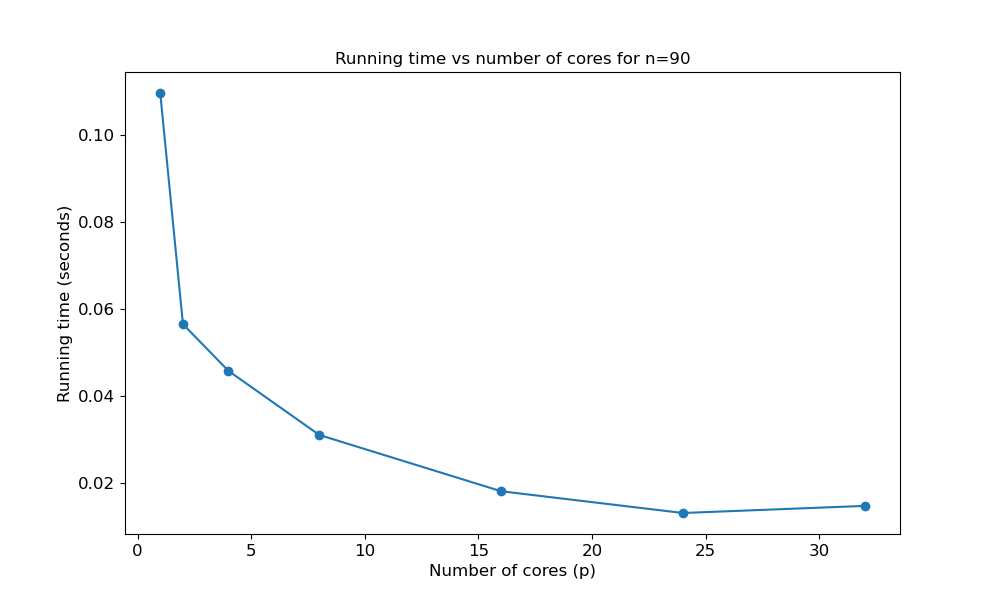
\includegraphics[width=0.75\textwidth]{./assets/juliap_job_90.png}
    \caption{Minimum runnting time vs number of cores for an input size of 90}
    \label{fig:juliap_job_90}
\end{figure}

\newpage
When setting the input size to 1100, figure~\ref{fig:juliap_job_1100} reveals that the running time decreases significantly up to 16 cores, similar to the n=90 case. Beyond 16 cores, the running time continues to decrease but at a much slower rate, and eventually stabilizes. Unlike the n=90 case, there is no noticeable increase in running time when using more than 24 cores, suggesting that the overhead is better managed or less impactful for larger workloads. The larger problem size of n=1100 benefits more from parallelization, as distributing the increased workload across multiple cores leads to more substantial performance gains.

\begin{figure}[htbp]
    \centering
    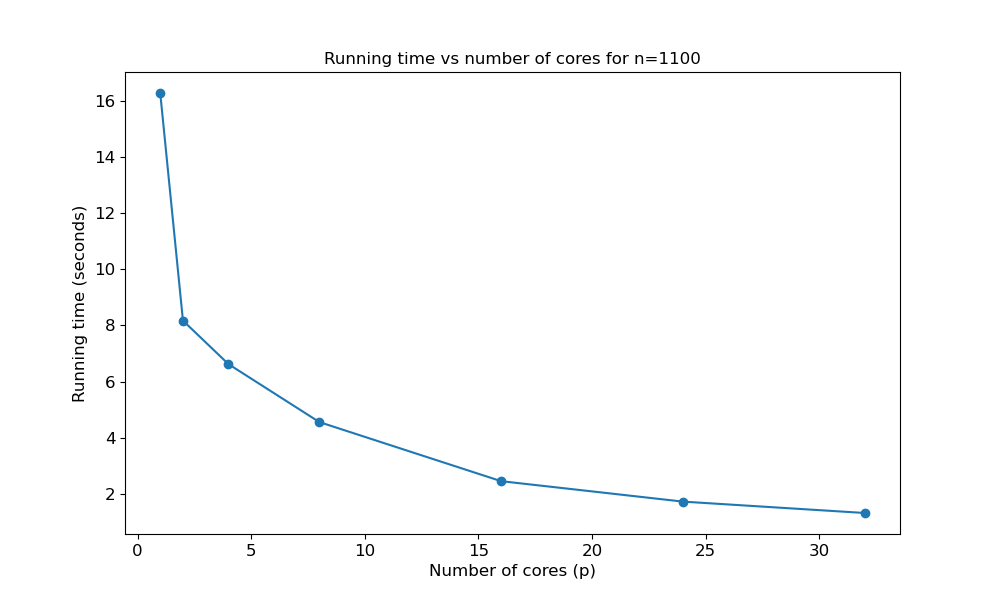
\includegraphics[width=0.75\textwidth]{./assets/juliap_job_1100.png}
    \caption{Minimum running time vs number of cores for an input size of 1100}
    \label{fig:juliap_job_1100}
\end{figure}

\subsection{Influence of schedule parameter}

The graph~\ref{fig:juliap2_job} demonstrates minimal differences in running times for different scheduling options with n=1100 and 16 cores. This suggests that the workload is well-balanced across the cores regardless of the schedule used which can also be confirmed by the previously discussed figure~\ref{fig:juliap_job_90} and figure~\ref{fig:juliap_job_1100}.  \texttt{Guided,8} performs slightly better than \texttt{dynamic,10} , likely due to better adjustment of chunk sizes. Both \texttt{static} and \texttt{static,1} schedules show similar performance, with \texttt{static,1} marginally better. Overall, the uniform nature of the workload leads to evenly distributed loads, making the scheduling overhead negligible.

\begin{figure}[htbp]
    \centering
    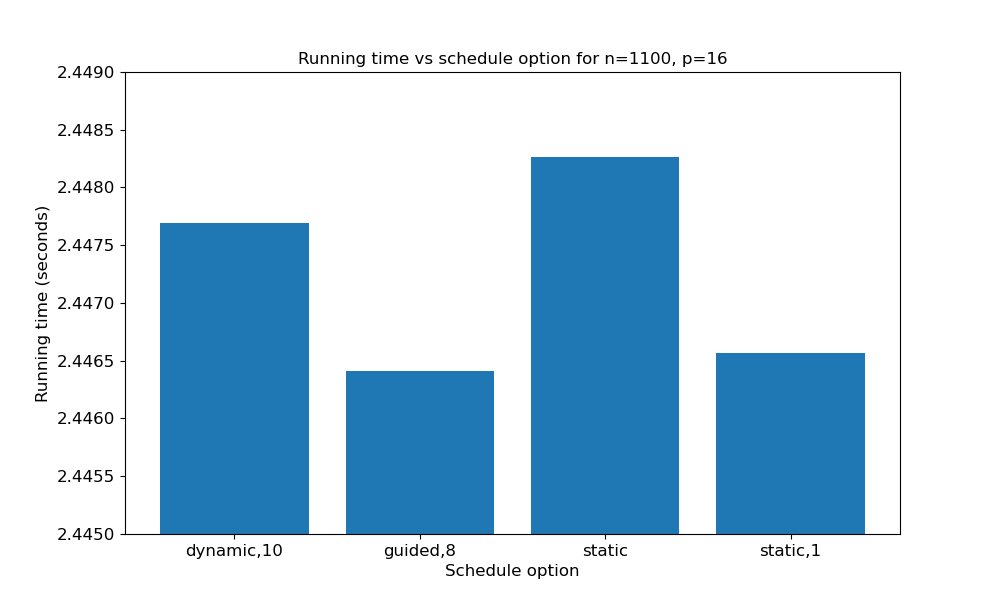
\includegraphics[width=0.75\textwidth]{./assets/juliap2_job.png}
    \caption{Minimum running time vs schedule option for an input size of 1100 and 16 cores}
    \label{fig:juliap2_job}
\end{figure}

% ----------------------------------------------------------------

\section{Exercise 6}

\subsection{Parallelize the filter computation}

Again, the thread team is created with \texttt{\#pragma omp parallel} and the tasks are created inside the parallel section. Without \texttt{single} each thread of the team would call \texttt{filter\_on\_pixel}. 
The private variables are initialized with the value of the outside variable, by defining them as \texttt{firstprivate} because otherwise all tasks created within the loop would reference the same i and j variables. The task-based parallelism would create a task for each pixel, which is why the block\_size was adapted and experimented with.

\subsection{Strong scaling analysis}

Figure~\ref{fig:strong_scaling_plot} shows that for a fixed problem size and varying the number of cores, the performance shows a clear trend where smaller block sizes (like 16) result in significantly higher running times as the number of cores increases. This sharp increase, especially noticeable at 32 cores, suggests that block size 16 is not well-suited for higher core counts. Larger block sizes (32 and 64) maintain relatively low running times with a gradual increase, indicating better parallel efficiency, likely due to reduced overhead and better cache utilization.  The optimal core range for block sizes 32 and 64 appears to be 16 to 24, where the running time is minimized.

\begin{figure}[htbp]
    \centering
    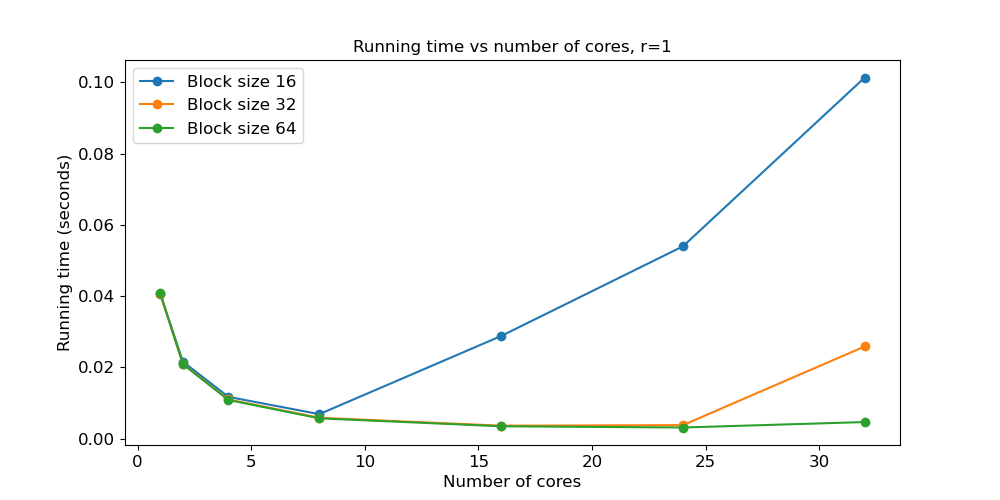
\includegraphics[width=0.75\textwidth]{./assets/strong_scaling_plot.png}
    \caption{Minimum running time vs number of cores for r=1 and various block sizes}
    \label{fig:strong_scaling_plot}
\end{figure}

\subsection{Weak scaling analysis}

In the weak scaling scenario, where both the number of cores and problem size increase proportionally, the running time should ideally remain constant if the system scales perfectly. However, as figure~\ref{fig:weak_scaling_plot} shows, the running time increases with a block size of 16 as there is a sharp increase indicating poor scalability and higher overheads as the workload grows. On the other hand, block sizes 32 and 64 exhibit much flatter curves, indicating better workload distribution. As a result, they provide a more stable and predictable performance across different core counts. 

\begin{figure}[htbp]
    \centering
    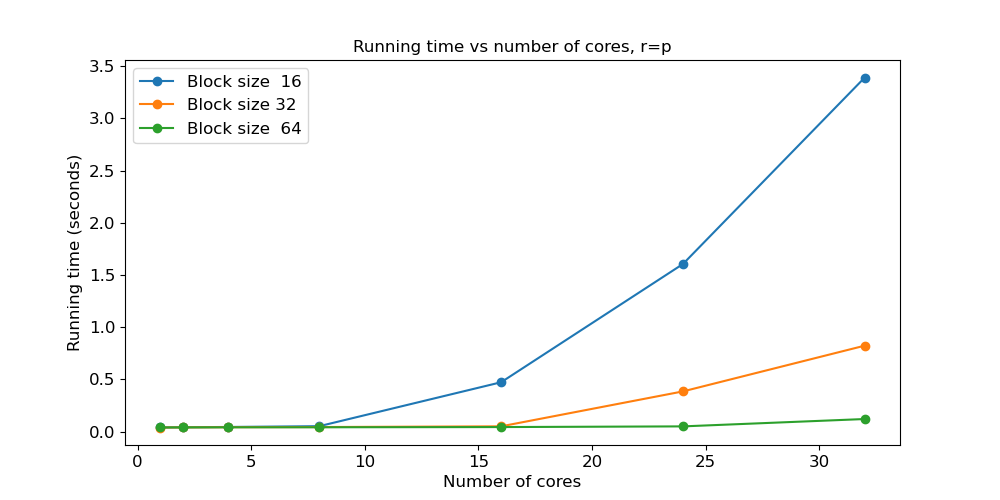
\includegraphics[width=0.75\textwidth]{./assets/weak_scaling_plot.png}
    \caption{Minimum running time vs number of cores for r=p and various block sizes}
    \label{fig:weak_scaling_plot}
\end{figure}

\newpage

\section{Appendix}

\begin{table}[htbp]
\centering
\csvautotabular{./output/juliap_job.csv}
\caption{julia strong scaling}
\label{tab:anotherlabel}
\end{table}

\begin{table}[htbp]
    \centering
    \begin{tabular}{|l|c|c|c|}
        \hline
        schedule & n & p & time \\
        \hline
        static & 1100 & 16 & 2.450491 \\
        static & 1100 & 16 & 2.448260 \\
        static & 1100 & 16 & 2.449136 \\
        static,1 & 1100 & 16 & 2.448672 \\
        static,1 & 1100 & 16 & 2.446850 \\
        static,1 & 1100 & 16 & 2.446568 \\
        dynamic,10 & 1100 & 16 & 2.447841 \\
        dynamic,10 & 1100 & 16 & 2.447689 \\
        dynamic,10 & 1100 & 16 & 2.453576 \\
        guided,8 & 1100 & 16 & 2.447433 \\
        guided,8 & 1100 & 16 & 2.447667 \\
        guided,8 & 1100 & 16 & 2.446407 \\
        \hline
    \end{tabular}
    \caption{julia schedule}
\end{table}

\begin{table}[htbp]
\centering
\csvautotabular{./output/filter_strong_job_16.csv}
\caption{filter strong scaling - blocksize = 16}
\label{tab:label1}
\end{table}

\begin{table}[htbp]
\centering
\csvautotabular{./output/filter_strong_job_32.csv}
\caption{filter strong scaling - blocksize = 32}
\label{tab:label2}
\end{table}

\begin{table}[htbp]
\centering
\csvautotabular{./output/filter_strong_job_64.csv}
\caption{filter strong scaling - blocksize = 64}
\label{tab:label3}
\end{table}

\begin{table}[htbp]
\centering
\csvautotabular{./output/filter_weak_job_16.csv}
\caption{filter weak scaling - blocksize = 16}
\label{tab:label4}
\end{table}

\begin{table}[htbp]
\centering
\csvautotabular{./output/filter_weak_job_32.csv}
\caption{filter weak scaling - blocksize = 32}
\label{tab:label5}
\end{table}

\begin{table}[htbp]
\centering
\csvautotabular{./output/filter_weak_job_64.csv}
\caption{filter weak scaling - blocksize = 64}
\label{tab:label6}
\end{table}

\end{document}
